\section{Μονοφασικός Αντιστροφέας Γέφυρας με μονοπολική PWM}
Μοντελοποιήθηκε ένας μονοφασικός αντιστροφέας γέφυρας με μονοπολική PWM τάσης εισόδου 100V και συχνότητα 50Hz στο οποίο εφαρμόζεται το ίδιο RL φορτίο (R = 10Ω, L = 0.025Η). Για την καλύτερη κατανόηση του, προσομοιώθηκε η λειτουργία του για $m_a = 0.9$ και $m_f = 40$  και $m_f = 200$ και καταγράφηκαν οι ακόλουθες κυματομορφές.

\subsection{Κυματομορφές Κυκλώματος}

\subsubsection*{Τάση και Ρεύμα εξόδου}
\begin{figure}[h!]
	\begin{subfigure}{0.49\textwidth}
		\centering
		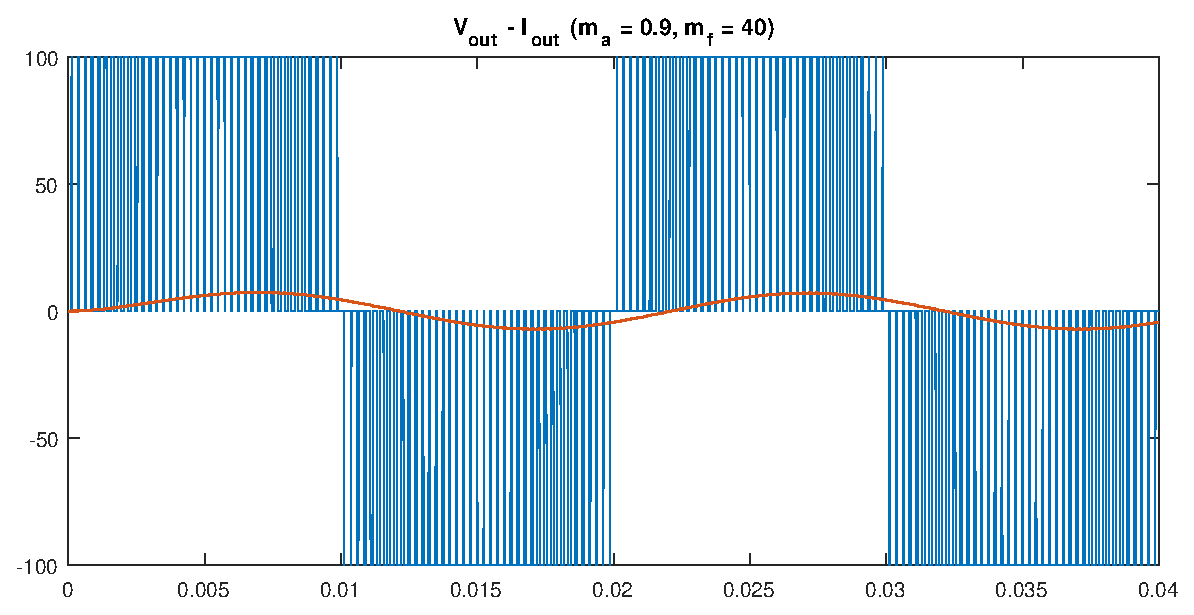
\includegraphics[width=1\textwidth]{Images/V_out_I_out_40}
	\end{subfigure}
	\begin{subfigure}{0.49\textwidth}
		\centering
		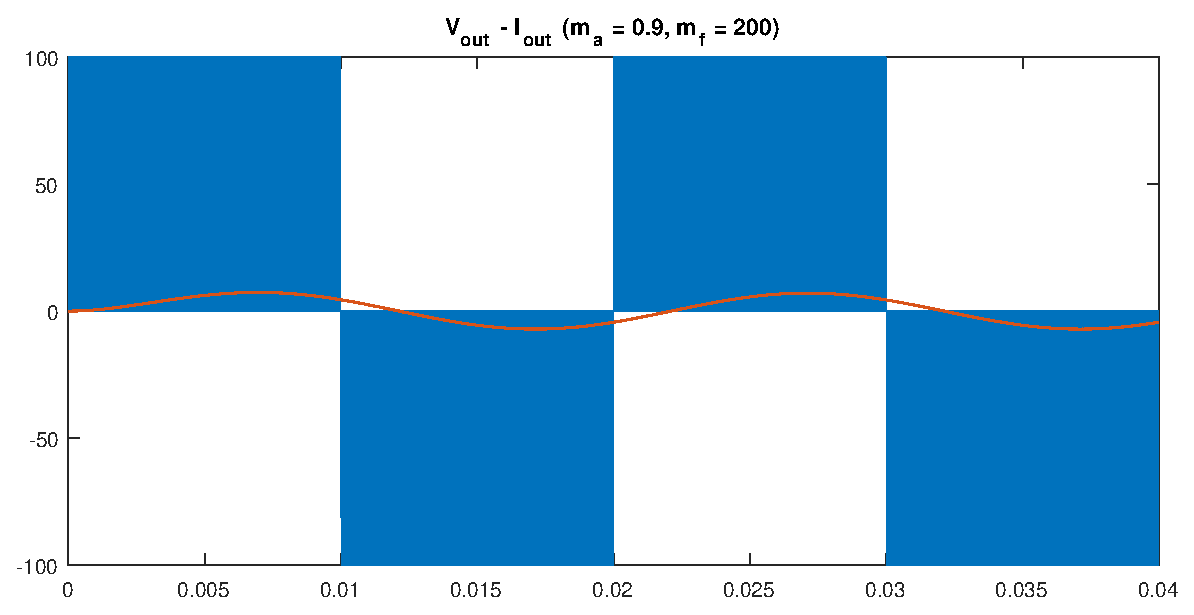
\includegraphics[width=1\textwidth]{Images/V_out_I_out_200}
	\end{subfigure}
	\noindent
	Σύμφωνα με τα παραπάνω figures, τόσο η τάση όσο και το ρεύμα εξόδου έχουν την αναμενόμενη μορφή, όπου το σήμα της τάσης αποτελείται από διακριτούς παλμούς και το ρεύμα εξόδου παρουσιάζει ημιτονοειδή μορφή.
	\subsubsection*{Τάση εξόδου}
	\begin{subfigure}{0.49\textwidth}
		\centering
		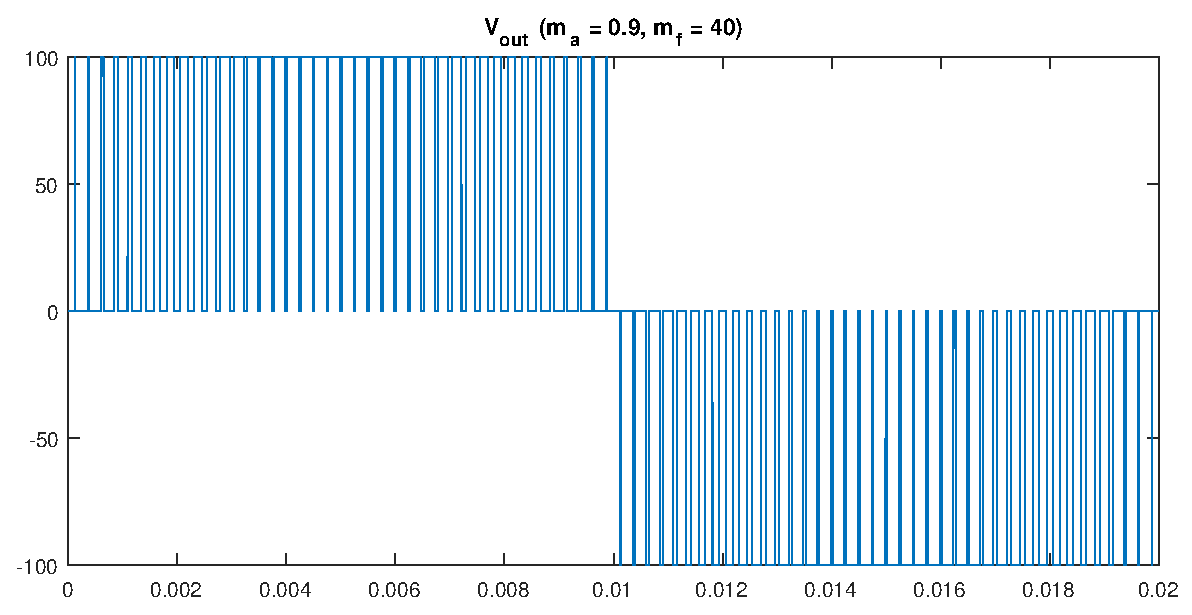
\includegraphics[width=1\textwidth]{Images/V_out_40}
	\end{subfigure}
	\begin{subfigure}{0.49\textwidth}
		\centering
		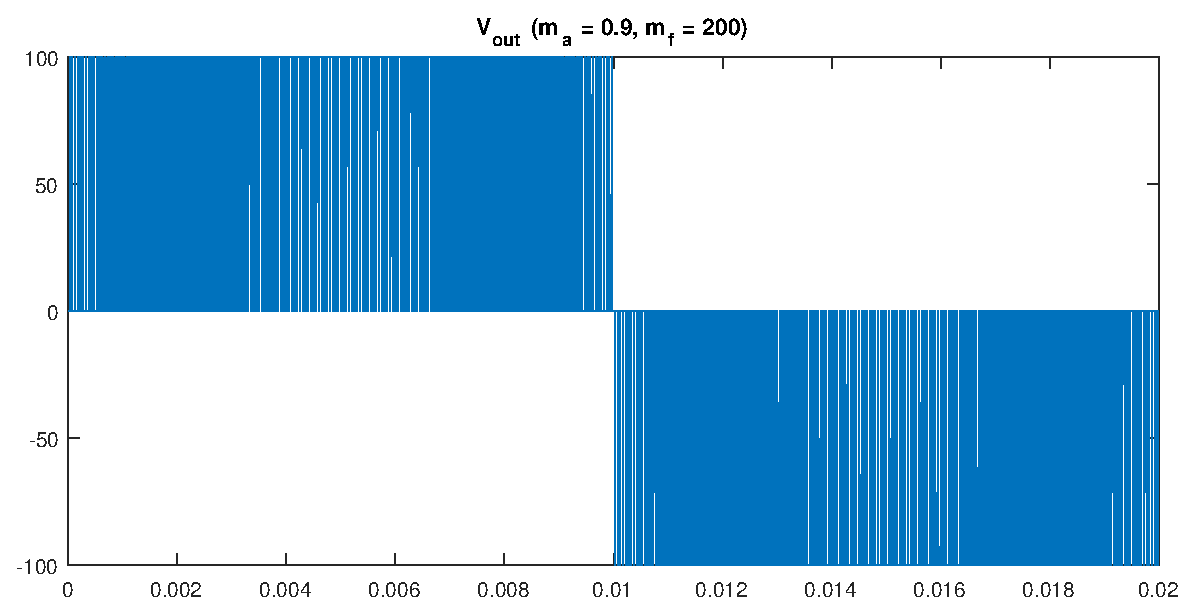
\includegraphics[width=1\textwidth]{Images/V_out_200}
	\end{subfigure}
\end{figure}
\noindent
Όσον αφορά την τάση εξόδου, αυξάνοντας τον $m_f$ παρατηρείται αύξηση του αριθμού των παλμών τάσης, συμπεριφορά  η οποία ήταν αναμενόμενη καθώς όπως προαναφέρθηκε στην υποενότητα \ref{single_PWM}, αυξάνοντας τον $m_f$ αυξάνεται ανάλογα η συχνότητα του τριγωνικού παλμού. Η αύξηση αυτή σε συνδυασμό με την σταθερή συχνότητα του επιθυμητού ημιτόνου, οδηγεί σε αύξηση των παλμών τάσης εφόσον αυτοί προκύπτουν μέσω σύγκρισης των δύο σημάτων.\\

\begin{figure}[h!]
	\subsubsection*{Ρεύμα εξόδου}
	\begin{subfigure}{0.49\textwidth}
		\centering
		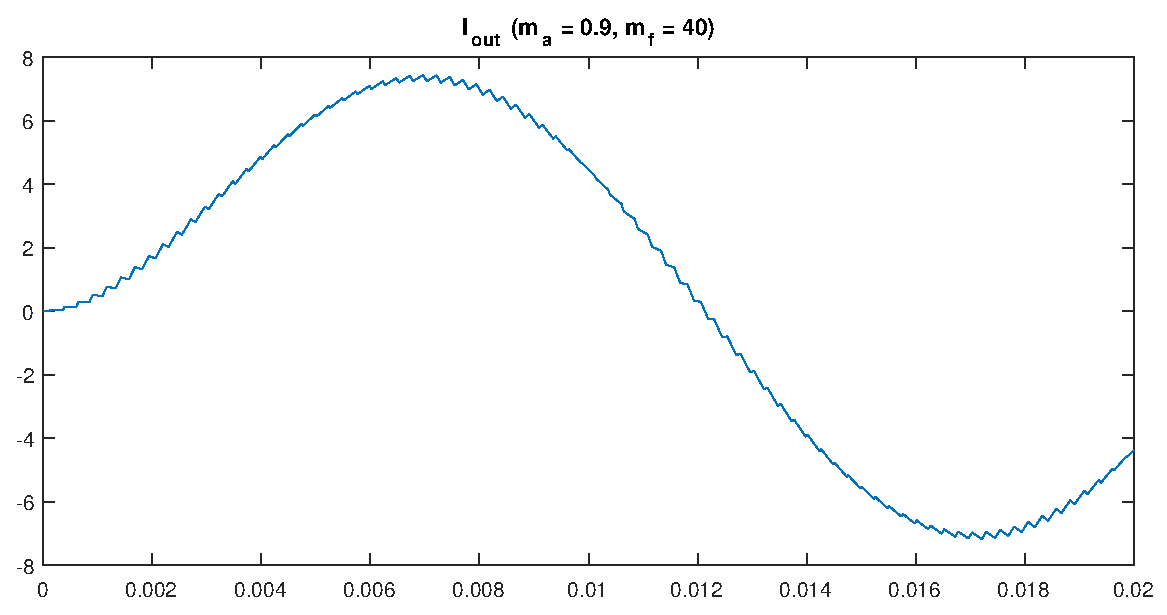
\includegraphics[width=1\textwidth]{Images/I_out_40}
	\end{subfigure}
	\begin{subfigure}{0.49\textwidth}
		\centering
		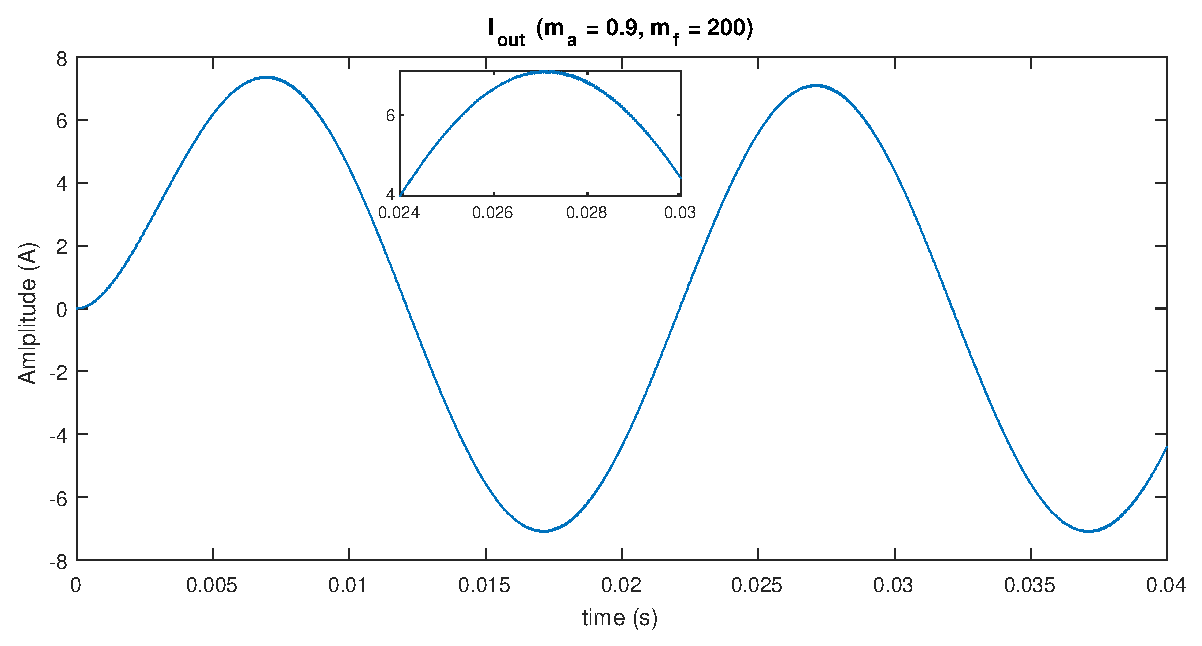
\includegraphics[width=1\textwidth]{Images/I_out_200}
	\end{subfigure}
\end{figure}
\noindent
Όσον αφορά το ρεύμα εξόδου, αυξάνοντας το $m_f$ παρατηρείται μείωση των διακυμάνσεων η οποία συνεπάγεται με μείωση των αρμονικών στο σήμα.\\\\
Η μείωση αυτή οφείλεται εν μέρη στο γεγονός πως το φορτίο είναι ωμικοεπαγωγικό και όπως είναι γνωστό, η σύνθετη αντίσταση του ισούται με $R + j\omega L$, οπότε αυξάνοντας τον $m_f$, αυξάνοντας πρακτικά την συχνότητα του φέροντος, αυξάνεται και η σύνθετη αντίσταση του μειώνοντας  έτσι την επίδραση των ανώτερων αρμονικών.

\noindent\\
 Ακόμη όπως προαναφέρθηκε (υποενότητα \ref{single_PWM}), αυξάνοντας τον $m_f$ οι αρμονικές του σήματος εμφανίζονται σε μεγαλύτερες συχνότητες με αποτέλεσμα να έχουν μικρότερη επιρροή.

\subsection{Συντελεστής Ισχύος}